\documentclass{article}
\usepackage{xeCJK}
\usepackage[utf8]{inputenc}
\usepackage{graphicx}
\usepackage{soul}
\usepackage{caption}
\usepackage[utf8]{inputenc}
\usepackage{amsmath}
\usepackage[dvipsnames]{xcolor}
\DeclareMathOperator*{\argmax}{arg\,max}
\DeclareMathOperator*{\argmin}{arg\,min}

\title{Estimation by the EM algorithm}
\author{Yun-Hsiang Chan}
\date{June 2021}

\begin{document}

\maketitle

A commonly used method of finding maximum-likelihood estimates of HMMs is the EM algorithm. The tools we need to do so are the forward and the backward probabilities. 

\section*{I. Forward and backwward probabilities}
Recall the row vector $\alpha_t$, for $t = 1, 2, ..., T$ as follows:
$$\alpha_t = \delta P(x_1) \Gamma P(x_2) ... \Gamma P(x_t) = \delta P(x_1) \Pi_{s=2}^t \Gamma P(x_s)$$
with $\delta$ denoting the initial distribution of the Markov chain. We have referred to the elements of $\alpha_t$ as \textbf{forward probabilities}, but we have not yet justified their description as probabilities. \\
\\
$\alpha_t(j)$, the jth component of $\alpha_t$, is indeed a probability, the joint probability $Pr(X_1 = x_1, X_2 = x_2, ..., X_t = x_t, C_t = j)$. \\
\\
We shall also need the vector of \textbf{backward probabilities} $\beta_t$ which , for $t = 1, 2, ..., T$ is defined by
$$\beta_t' = \Gamma P(x_{t+1}) \Gamma P_{x_{t+2}} ... \Gamma P(x_T) 1' = (\Pi_{s=t+1}^T \Gamma P(x_s)) 1'$$
with the convention that an empty product is the identity matrix; the case $t = T$ therefore yields $\beta_T = 1$. \\
\\
$\beta_t(j)$, the jth component of $\beta_t$, can be identified as the conditional probability $Pr(X_{t+1} = x_{t+1}, ..., X_T = x_T | C_t = j)$. \\
\\
It will then follow that, for $t = 1, ..., T$
$$\alpha_t (j) \beta_t (j) = Pr(X^{(T)} = x^{(T)}, C_t = j)$$

\subsection*{1. Forward probabilities}
It follows immediately from the definition of $\alpha_t$ that , for $t = 1, ..., T-1$, $\alpha_{t+1} = \alpha_t \Gamma P(x_{t+1})$ or, in scalar form, 
$$\alpha_{t+1}(j) = (\sum_{i=1}^m \alpha_t(i)\gamma_{ij}) p_j(x+1)$$
\\
\textbf{Proposition 1} \\
For $t = 1, ..., T$ and $j = 1, ..., m$
$$\alpha_t(j) = Pr(X^{(t)} = x^{(t)}, C_t = j)$$
\\
The proof is in Figure 1.
\begin{figure}
    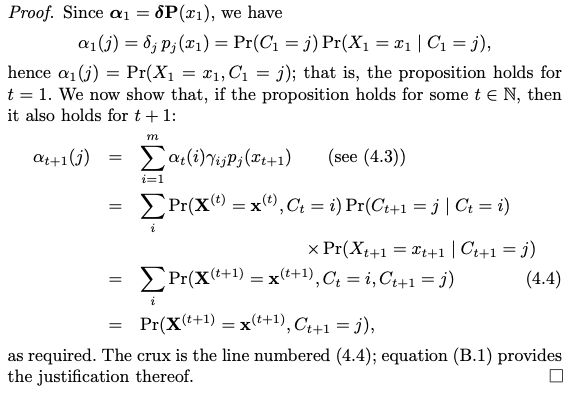
\includegraphics[width = 10cm]{prop 2.png}
    \caption{Proof of Proposition 1}
\end{figure}

\subsection*{2. Backward probabilities}
It follows immediately from the definition of $\beta_t$ that $\beta_t' = \Gamma P(x_{t+1}) \beta_{t+1}'$, for $t = 1, ..., T-1$ \\
\\
\textbf{Proposition 2} \\
For $t = 1, ..., T - 1$, and $i = 1, 2, ..., m$
$$\beta_t(i) = Pr(X_{t+1} = x_{t+1}, X_{t+2} = x_{t+2}, ..., X_T = x_T | C_t = i)$$
providied that $Pr(C_t = i) > 0$. In a more compact notation,
$$\beta_t(i) = Pr(X_{t+1}^T = x_{t+1}^T | C_t = i)$$
where $X_a^b \text{ denotes the vector } (X_a, X_{a+1}, ..., X_b)$
\\
\\
This proposition identifies $\beta_t(i)$ as a conditional probability: the probability of the observations being $x_{t+1}, ..., x_T$, given that the Markov chain is in state $i$ at time $t$. \\
\\
The entire proof is in the textbook.

\subsection*{3. Properties of forward and backward probabilities}

We now establish a result relating the forward and backward probabilities $\alpha_t(i)$ and $\beta_t(i)$ to the probabilities $Pr(X^{(T)} = x^{(T)}, C_t = i)$. This we shall use in applying the EM algorithm to HMMs, and in local decoding. \\
\\
\textbf{Proposition 3} \\
For $t = 1, ..., T$ and $i = 1, ..., m$
$$\alpha_t(i) \beta_t(i) = Pr(X^{(T)} = x^{(T)}, C_t = i)$$
and consequently $\alpha_t \beta_t' = Pr(X^{(T)} = x^{(T)} = L_T)$, for each such $t$. \\
\\
\textbf{Proposition 5} \\
Firstly, for $t = 1, ..., T$
$$Pr(C_t = j | X^{(T)} = x^{(T)}) = \alpha_t(j) \beta_t(j) / L_T$$
and secondly, for $t = 2, ..., T$
$$Pr(C_{t-1} = j, C_t = k | X^{(T)} = x^{(T)}) = \alpha_{t-1}(j) \gamma_{jk} p_k(x_t) \beta_t(k) / L_T$$

\section*{The EM algorithm}






\end{document}